\chapter{Computing thermal conductivity} 

\label{Chapter2} 

In Chapter~\ref{Chapter1}, I introduced the key concepts surrounding this study. I will be investigating the magnitude of thermal conductivity throughout the deep Earth, considering the effect of physical conditions and Fe impurities. I will be using computational approaches to access this parameter, as experiments are difficult to perfrom in the regime I require. 

Part of computing results is ensuring the simulations are running faithfully to the material of interest and the physical processes that operate in bulk materials. In this chapter I introduce the background to calculating conductivity through simulation, and show fundamental system setup and parameter convergence. 

The following chapters apply theory introduced here to investigate how conductivity is affected by; system shape and size, and adding impurities to an otherwise regular crystal structure.

%-----------------------------------------------------------
\section{Atomic-scale modelling}
%-----------------------------------------------------------

!!! THIS SECTION HAS REDUNDANCY WITH ABOVE CHAPTER INTRO SPIEL

!!! PROBABLY REVISE HEAVILY

Knowledge of thermal conductivity is important for modelling the deep earth, but can not be measured experimentally at core mantle boundary conditions. Atomic scale simulations sidestep experimental limitations, but system size must be chosen carefully in order to determine accurate conductivity values. 

A range of atomic scale simulation methods are available to determine the lattice thermal conductivity of materials. These are invaluable for calculating thermal conductivity at conditions of which experiments are difficult, e.g. the extreme conditions found in the Earth's lower mantle (pressures and temperatures up to 136~GPa and 4000~K at the core-mantle boundary). 

%---------------------------------------
\subsection{Computational approaches (for modelling atoms...?)}
%---------------------------------------

Before you can calculate material properties of interest, you need to determine how the atoms will interact with one another in your system. I do not mean the magnitude of the interactions or the parameters you choose to replicate a material, but the specific theoretical approach of atomic-scale modelling. There are multiple regimes for doing so, a couple of which are described below.

%-------------------
\subsubsection{Molecular dynamics}
%-------------------

In a moldecular dynamics (MD) calculation, atoms in a simulation cell have masses, velocities, and forces acting between them. At each computational timestep the net force on each atom is calculated from all the other atoms. Accelerations are then calculated from Newton's second law of motion, which are used to update the velocities and positions of the atoms. The process is repeated, iteratively updating parameters every timestep. At zero temperature, a parameter such as unit cell volume will converge, but this is not true when finite temperatures are considered. Temperature fluctuations mean cell volume will constantly change, regardless of simulation length. The solution is to take the cumulative average over many timesteps, which converges eventually.

!!! FLOWCHART FIGURE, MD TIMESTEP PROCESS?

%-------------------
\subsubsection{Lattice dynamics}
%-------------------

An alternative approach to MD is lattice dynamics (LD),where the response of all atoms to the motion of one is considered. Each atom in the simualtion cell is perturbed in turn, the motions and response of the other atoms stored  in a 3 by 3 tensor for each atom pairing. The tensor takes significant time to compute compared to a single MD timestep, but can be used to calculate various material properties once obtained. The focus of this study will be on MD approaches, but LD results from literature will be reviewed for comparison.

!!! ADD A REFERENCE AND FORGET ABOUT IT?

!!! DO I NEED TO SAY WHY I AM NOT USING LD? WHY AM I NOT USING LD!?














%---------------------------------------
\subsection{Calculating atomic interactions}
%---------------------------------------

!!! ADD INTRO SPIEL HERE

%-------------------
\subsubsection{Density functional theory}
%-------------------

Density functional theory (DFT) is a way of determining accurate interatomic forces. The properties of the electrons are considered along with the nuclei, which increases the computational cost and simulation run time. This additionally limits the size of systems, or number of atoms (on the order of thousands), that can be considered. Calculating from first principles in this manner should only be considered if you know the system parameters for converged results, and they can be completed on a suitable timescale. I will be opting for a different approach, as I wish to investigate a large amount of big systems systems, potentially for multiple compositional variations.

!!! ANY OTHER ALTERNATIVE APPROACHES THAT NEED TO GO HERE?

%-------------------
\subsubsection{Classical interatomic potentials}
%-------------------

The alternative to DFT is to use empirically-derived potentials to calculate the interatomic forces. Whereas calculating from first principles considers the interactions of atoms and their outer shell electrons, interatomic potentials use an approximation of the electronic potential component (i.e. a classical atomic model). 

Systems on the order of millions of atoms can be considered with atomic potentials, due to significantly reduced computational cost compared to DFT. The trade-off is accuracy however, which is controlled by the characteristics of the employed potential. These potentials are set up to reproduce a set of experimental results, but the is no certainty they reflect true values outside their calibrated range of conditions. A realsitic model reproduces the structural, elastic, and thermal properties of a material. A common feature of classical potentials is to underestimate the diagonal terms of the elastic constant tensor, and overestimate the off-diagonal, where the discrepancy increases with pressure \citep{Chen2012}.

%-------------------
\subsubsection{Oganov's \bdgs potential}
%-------------------

The interatomic potential I will be using  was developed by \citet{Oganov2000}. Many potentials exist for \mgsios perovskite, but the aforementioned is robust up to lower mantle pressures and temperatures. The interatomic potential function includes ionic, covalent, and van der Waals components. The dominant long-range term is the Coulomb interaction, and the short-range interactions are described using a Buckingham potential with the Born-Mayer potential, and a $C/r^{6}$ van der Waals term. The equation for pair-wise potential (summed for potential energy of the system) takes the form
%
\begin{equation}
V_{ij}^{\mathrm{Buck}}
= \frac{1}{4 \pi \epsilon_{0}} 
\frac{q_{i} q_{j}}{r_{ij}} 
+ b_{ij}\ exp\left ( \frac{-r_{ij}}{\rho_{ij}} \right )
- \frac{c_{ij}}{{r_{ij}}^{6}} \  ,
\label{eq.buck}
\end{equation}
%
where $q_{i}$ and $q_{j}$ are the charges of atoms $i$ and $j$, $r_{ij}$ is the distance between them, $b_{ij}$ is the pre-exponential repulsive parameter for the pair, $\rho_{ij}$ is the repulsion exponent, and $c_{ij}$ is the van der Waals parameter.
There are three sets of these paramters, for each of the interacting atomic pairs (shown in Table~\ref{tab.oganov}). The charges for Mg, Si, and O atoms are $1.9104$, $2.9043$, and $-1.6049$, respectively.
%
\begin{table}[h]
\centering
\caption[CONTENTS BIT]{\label{tab.oganov}Parameters used to define \citet{Oganov2000}'s \mgsios perovskite potential.}
\begin{tabular}{clll} 
Bond $ij$ & $b_{ij}$ (eV)  & $\rho_{ij}$ (\AA) & $c_{ij}$ (eV.\AA$^{6}$) \\ \hline
Mg-O        & 1041.435        & 0.2866                 & 0                \\
Si-O          & 1137.028        & 0.2827                 & 0                \\
O-O          & 2023.800        & 0.2674                  & 13.83         \\ \hline       
\end{tabular}
\end{table}



%-------------------
\subsubsection{SETTING UP POTENTIAL CUTOFFS}
%-------------------

Part of applying classical potentials is setting up the distance over which they act, the maximum seperation between two atoms before they are not paired for force calculation. Too small a cut-off distance, and the material is not being replicated faithfully. Too large a cut-off, you are performing more calculations than you need, and will increase computation time. The potential between two atoms is inversely proportional to their separation (see Eq. \ref{eq.buck}), ``cutting off'' in this manner is acceptable when the value is tending towards zero with large interatomic distance. I consider two cut-off distances, for both the Coulombic and the Buckingham interactions (the former have a larger value than the latter).

 !!! BUT WHAT DID I DECIDE ON THOUGH 











%---------------------------------------
\subsection{Finite-size effects}
%---------------------------------------

Computational techniques are not limited by the reproduction of physical conditions like experiments, this does not mean they are without limitations however. Finite-size effects refer to when the number of atoms or system shape and size affect the computed result, compared to an infinite system. In the case of thermal conductivity, the problem arises when phonons are truncated by boundaries in the simulation cell. As discussed in Chapter~\ref{sec.phonon_explan}, phonons have wave-like properties, including wavelength. 

When a simulation cell is shorter than a phonon, that phonon cannot be represented in the system. This will mean a calculation is tending to underestimate conductivity. The opposite scenario is also true, if the phonon mean free path is longer than the distance between boundaries in a system, phonon scattering behaviour is not being replicated accurately. This leads to overestimations, where phonons are able to transport heat unimpeded, and conductivity is strongly dependent on system size \citep{Tadano2014}. 

The FSE observed for a material change with thermal conductivity/phonon MFP, and thus are pressure, temperature, and composition sensitive. Long MFPs require larger systems to eliminate FSE (and vice versa) [[[BUT IS THIS TRUE?]]].

This can be a problem when employing DFT calculations, where systems sizes must be kept small to maintain computational efficiency. Testing system size is also a problem, as calculations of large systems must be performed to check convergence of results.

%-------------------
\subsubsection{LAMMPS}
%-------------------

LAMMPS (Large-scale Atomic/Molecular Massively Parallel Simulator) is a classical molecular dynamics code \citep{Plimpton1995}. I will be using it to look at large systems (up to the order of $10^5$ atoms) and assess how size and shape affects results. While calculations using interatomic poternials are not as accurate as those using DFT, a main focus of this work will be on the observations of conductivity magnitude change between systems of varying size. The \wmks result isn't as important as confirming phonon behaviour is not being greatly inhibited. 

While not considered here, the system size parameters I determine for \bdgs at a range of temperatures and pressures could be used in a DFT calculation. This ensures the DFT calculation is using a large enough arrangement of atoms, while providing a useful reliability check for my classical results. 

















\pagebreak
















%-----------------------------------------------------------
\section{Computing \tc}
%-----------------------------------------------------------

I will be using two approaches, both utilising classical interatomic potentials, to calculate thermal conductivity throughout this thesis. They will be explained later in this section, and are as follows,

(1) The non-equilbrium molecular dynamics-based ``direct method'', where thermal conductivity is calculated from an imposed heat flux and corresponding temperature gradient via Fourier's Law \citep{Muller-Plathe1997,Nieto-Draghi2013}.

(2) Equilibrium molecular dynamics based on the Green-Kubo relations to determine the thermal conductivity from heat flux fluctuations and their time-dependence \citep{Green1954,Kubo1957,Kubo1966,Schelling2002}. 


\citet{Stackhouse2010} review other methods to compute thermal conductivity, including the above but also,

(3) Anharmonic lattice dynamics \citep{Tang2009}. %(BTE)CHERNATYNSKIY and PHILLPOT 2010?

(4) Combined quasiharmonic lattice dynamics and molecular dynamics method \citep{DeKoker2009}.

!!! Fixed ends? Sinusoidal temperature perturbation?

The Green-Kubo and direct method use the same underlying atomic model, but calculate \tcs differently. They have their own unique system setup procedures, data processing work flows, and finite-size effects. In the following sections, each method will be considered individually, before a review of literature comparing the two, and how I will use them to analyse their FSE.



%---------------------------------------
\subsection{Direct method}
%---------------------------------------
The direct method is the computational implementation of a typical experiment to measure thermal conductivity, using Fourier's law to relate heat flux ($q$) and temperature gradient ($\nabla{T}$) to thermal conductivity ($k$), 
%
\begin{equation}
q=-k \nabla{T} 
\label{fourier}.
\end{equation}

%-------------------
\subsubsection{System setup}
%-------------------

In the direct method energy is transferred from one group of atoms to another, creating hot and cold regions between which heat flows. The resultant temperature gradient is measured by calculating the temperature of individual groups of atoms along the direction of the heat flux. Simulation cells tend to be long relative to their cross-sectional area, defined as height by width (see Figure~\ref{fig:cell_dia}). Cell boundaries are periodic and the hot and cold sections are half the cell length apart, meaning heat flows in both directions from hot to cold (one of which is across the length-end periodic boundary). This results in two similar temperature gradients which can be averaged.

\begin{figure}[h]
  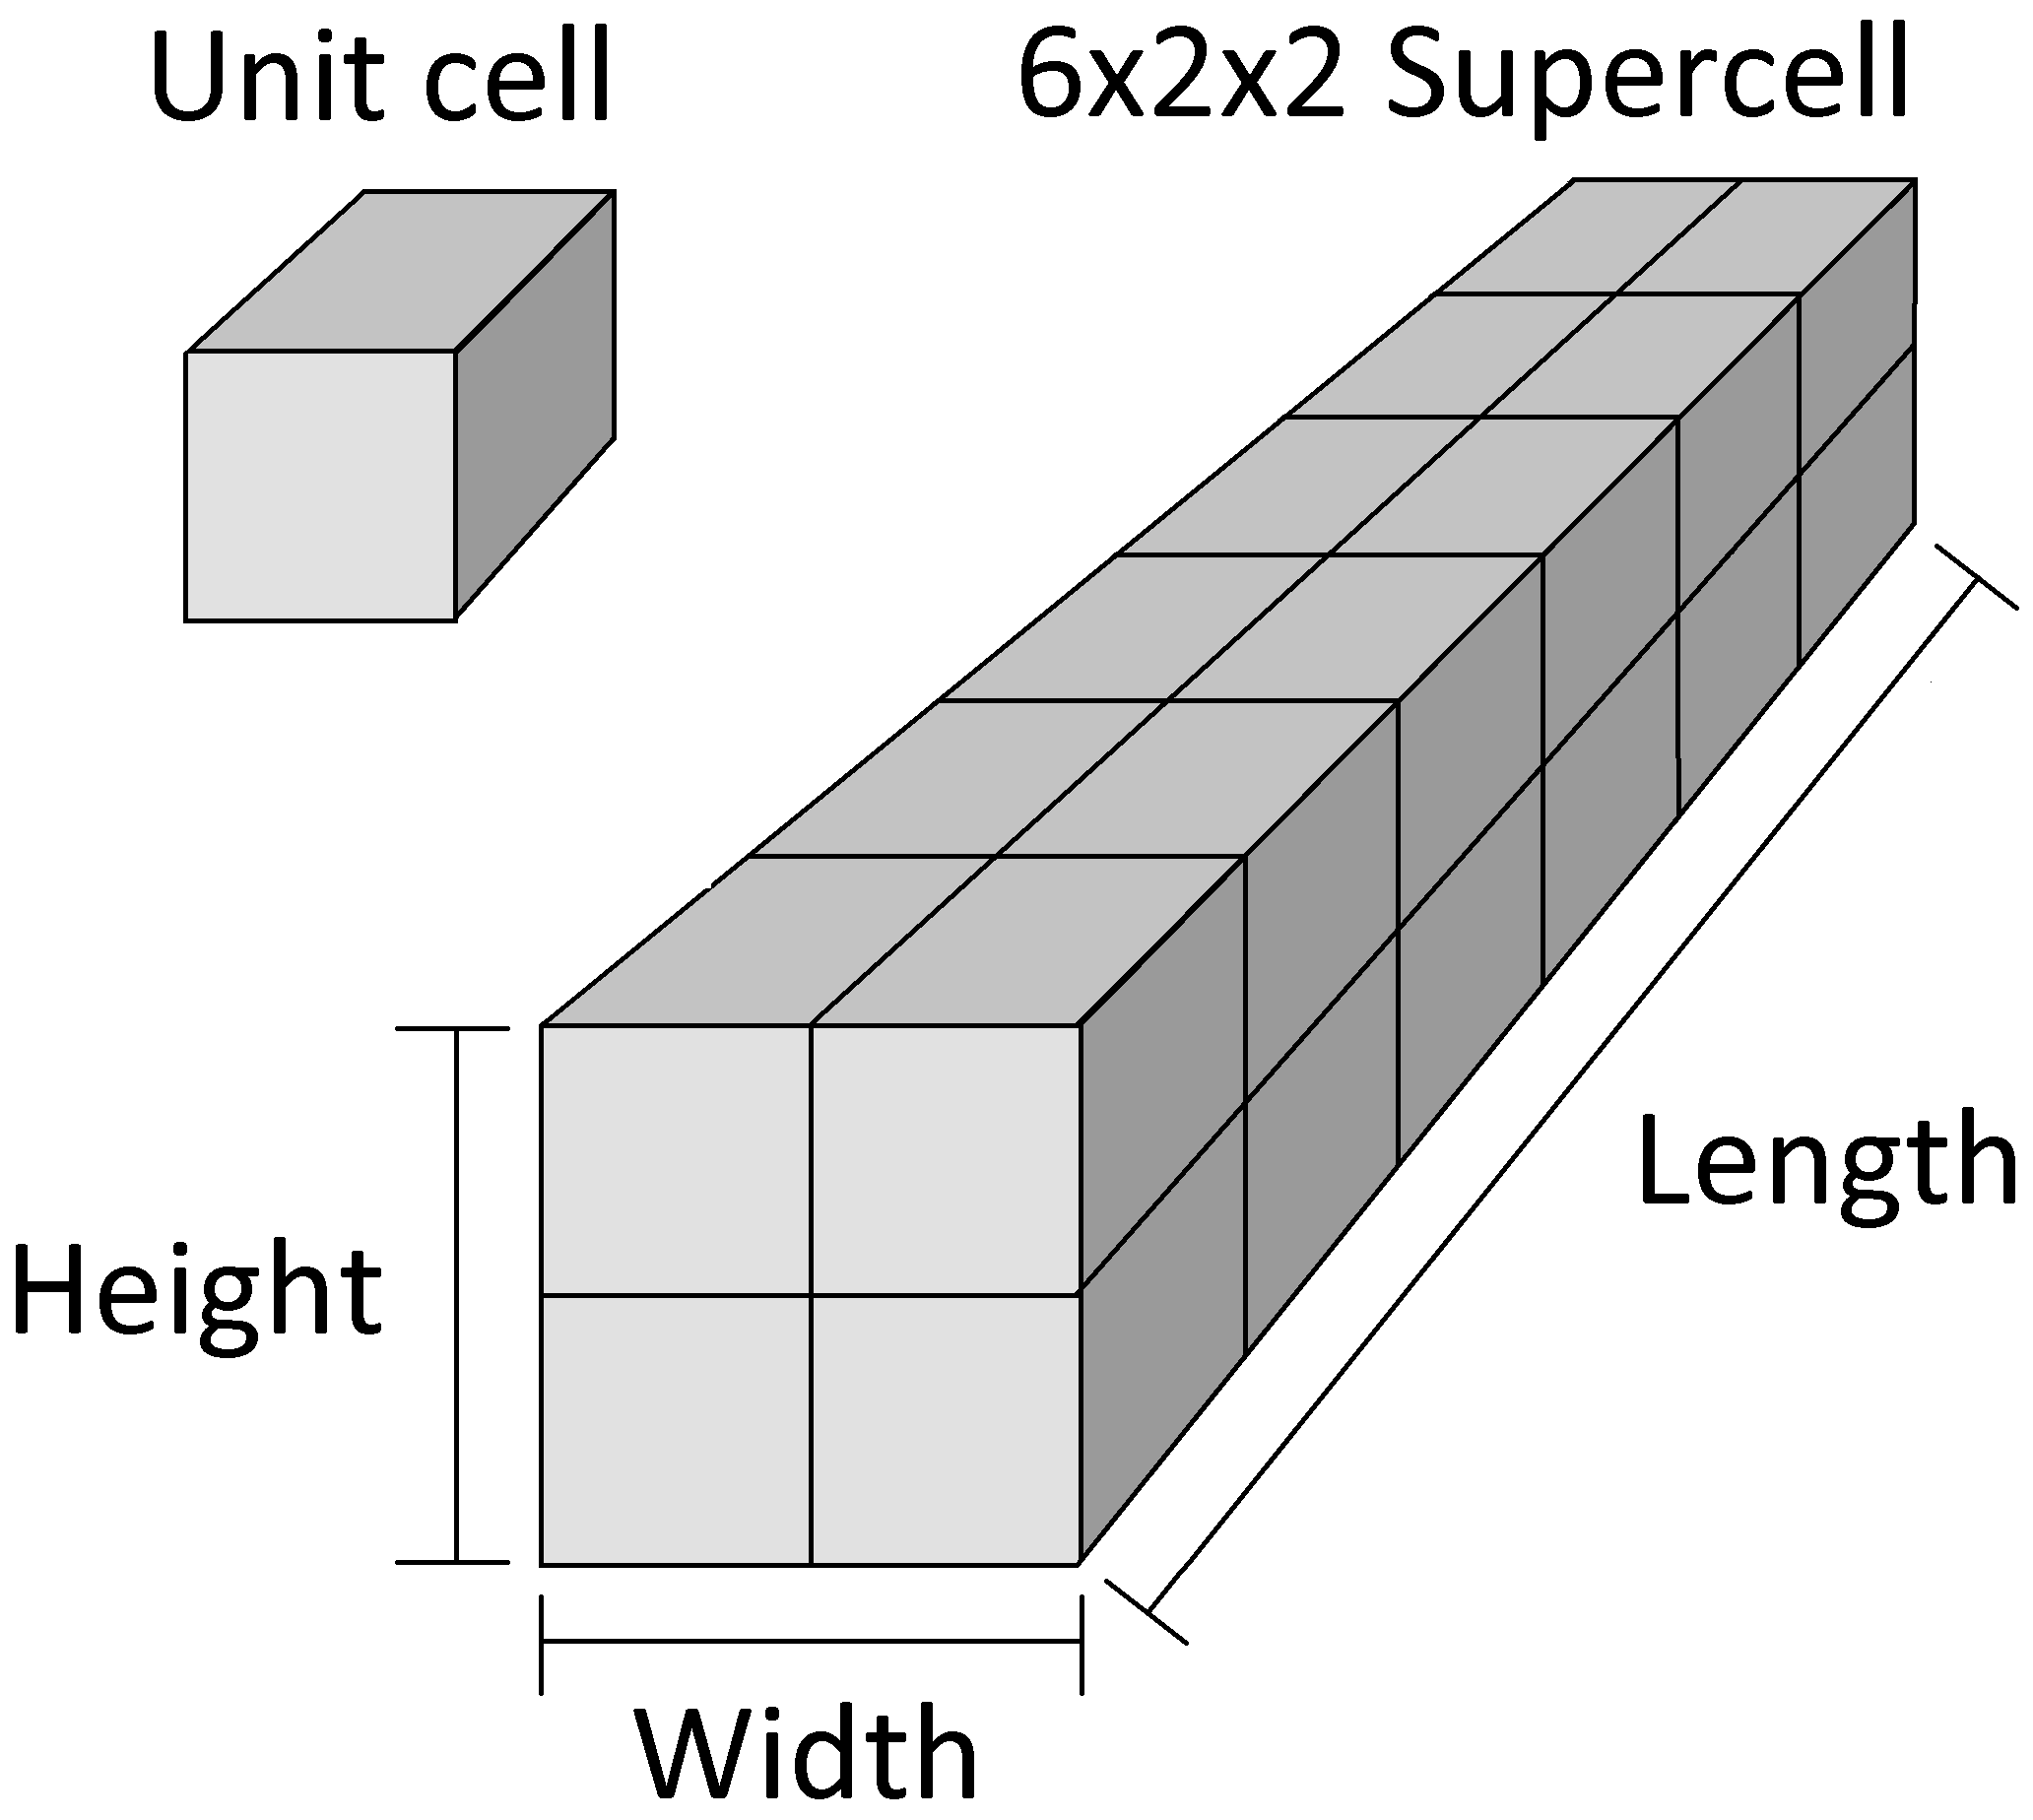
\includegraphics[width=\linewidth]{Figures/cell_diagram.png}
  \caption{The unit cell represents the smallest box of atoms that can be replicated to produce a crystal structure. A supercell is an arrangement of unit cells.}
  \label{fig:cell_dia}
\end{figure}

\begin{figure}[h]
  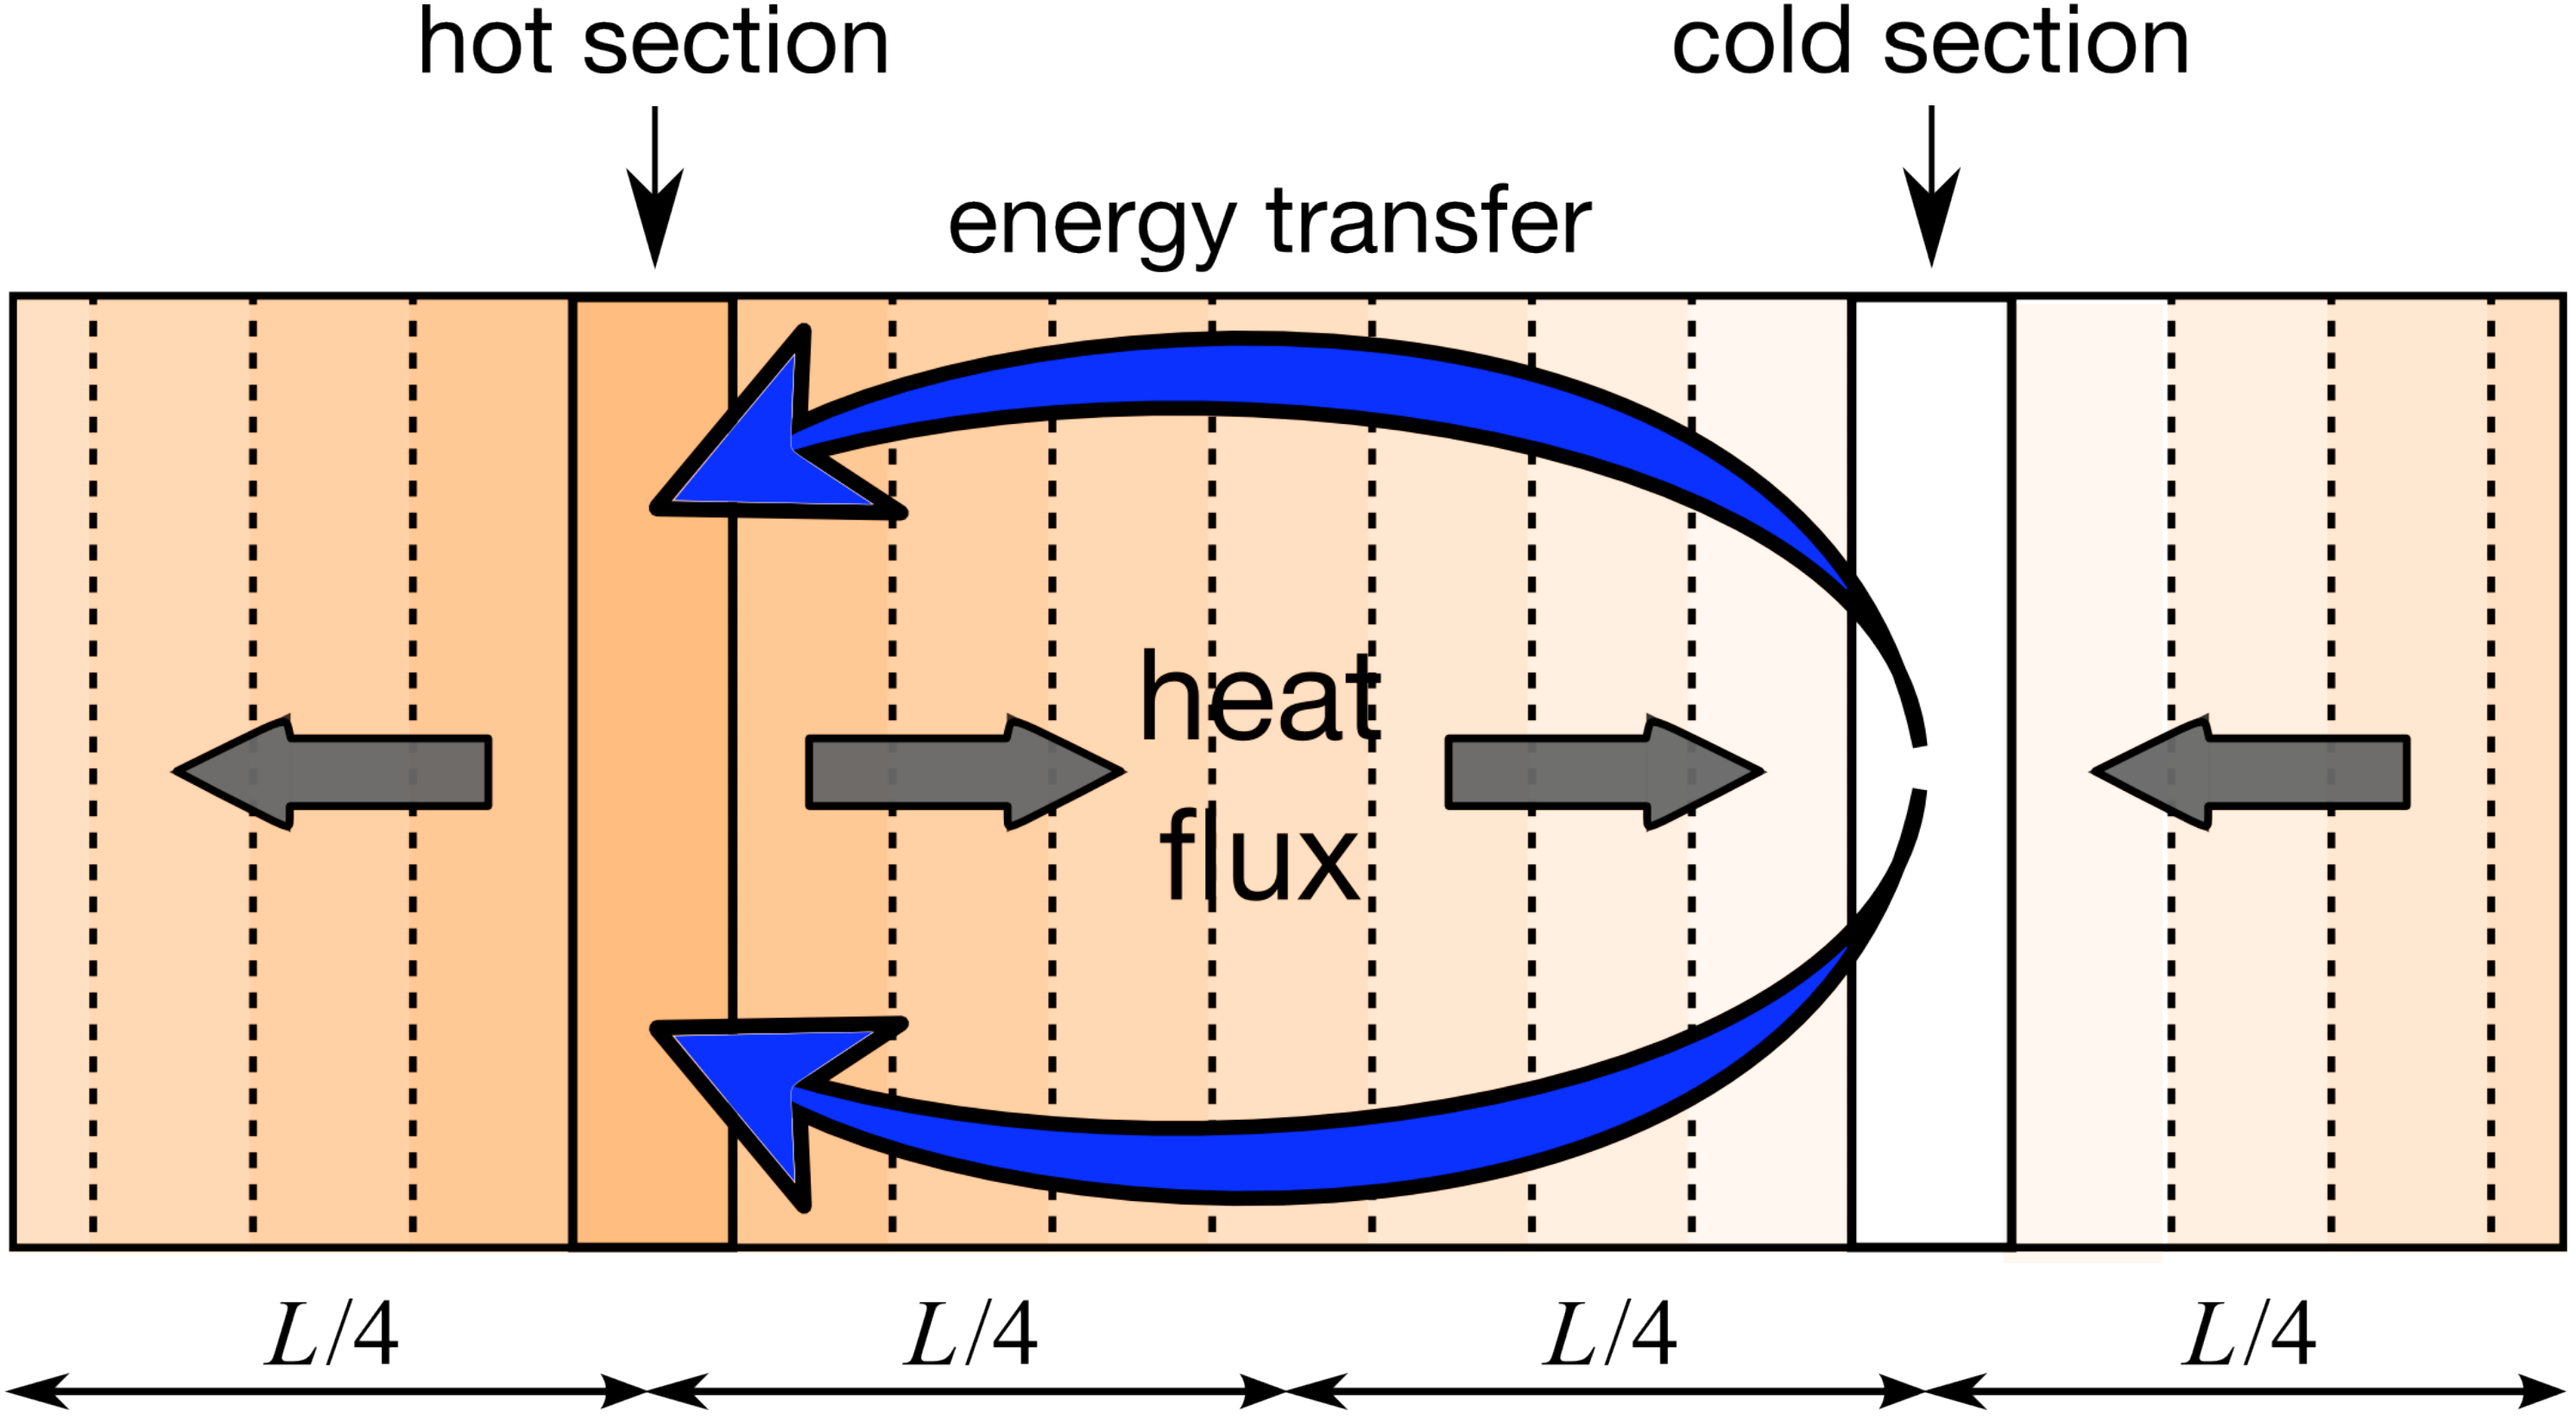
\includegraphics[width=\linewidth]{Figures/ss_direct_mod.png}
  \caption{Movement and distribution of heat in the direct method. Orange to white scale represents temperature \citep[modified from][]{Stackhouse2015}.}
  \label{fig:ss_direct}
\end{figure}

From kinetic theory [[[REF?]]], conductivities computed by the direct method ($k_L$) are dependent on length of simulation cell,
\begin{equation}
k_{L} = \frac{1}{3} C_{V} v l_{L} \label{length-dep},
\end{equation}

where $C_v$ is the volumetric heat capacity, $v$ is the average phonon drift velocity, and $l_L$ is the phonon mean free path. 

%-------------------
\subsubsection{Data processing}
%-------------------

The finite size of the simulation cell truncates the mean free path, underestimating conductivity compared to that of the bulk material ($k_\infty$). Using results from simulations of varying cell length ($L$), conductivity is extrapolated to a length-independent value (where $b$ is a material dependent parameter),

\begin{equation}
{k_{L}}^{-1} = b L^{-1} + {k_{\infty}}^{-1} \label{linear-extrap}.
\end{equation}

Inverse conductivities from direct method simulations are plotted against corresponding inverse cell lengths. A straight line is fit to the data and extrapolated to the y-axis (at which the inverse cell length equals zero and real length equals infinity), where the intercept gives the inverse of the bulk material conductivity \citep{Schelling2002}.

\begin{figure}[h]
  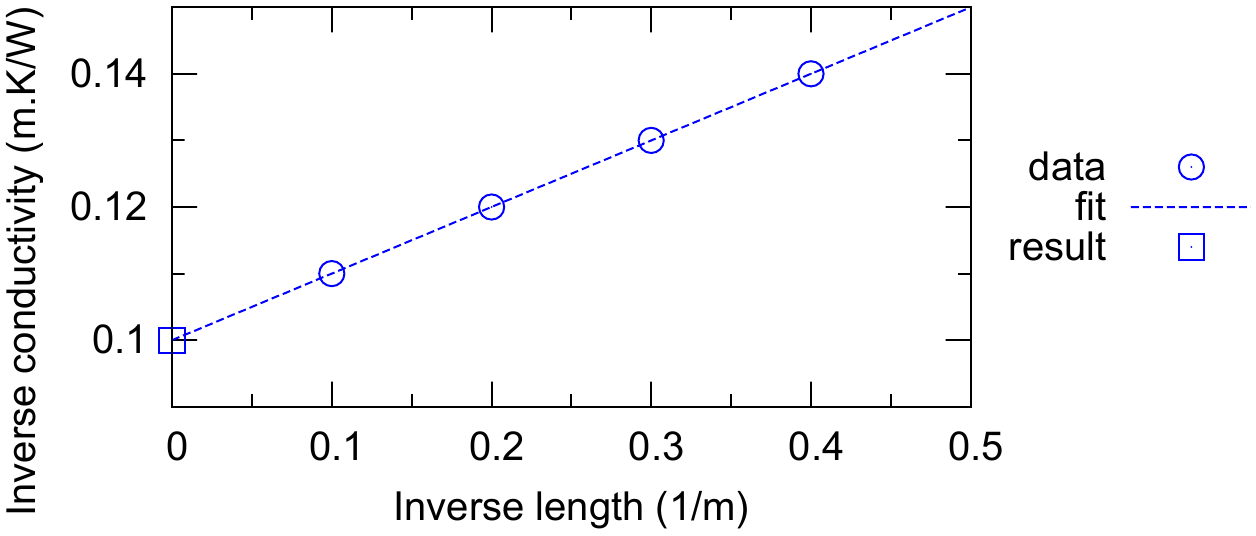
\includegraphics[width=\linewidth]{Figures/ideal_extrap.png}
  \caption{Idealised example of linear extrapolation procedure. Inverse computed conductivities are plotted against inverse simulation lengths. Extrapolation to y-axis gives conductivity of an infinite system length, i.e. the bulk material.}
  \label{fig:ideal}
\end{figure}

%-------------------
\subsubsection{Finite-size effects}
%-------------------

Problems arise when the data do not support a linear trend. There are two effects of finite system size that can cause an individual direct method simulation to diverge away from an inferred/expected linear trend, both of which result in overestimation of the length-dependent conductivity data point. First, when the distance between hot and cold sections (controlled by cell length) is shorter than the MFP, phonons travel ballistically (i.e. without any scattering events) from heat source to sink \citep{Sellan2010}. Conductivites in shorter length cells are overestimated when this occurs, reducing the gradient of the linear fit and thus underestimating the extrapolated conductivity.

For a given length, conductivity is dependent on the CSA, or aspect ratio of the simulation cell. Conductivity is overestimated due to an underestimation of phonon-phonon scattering, from sparse phonon phase sampling in cells where cross-section is small compared to length. Phonons that aren't resolved cannot contribute to phonon-phonon scattering effects. Reduced scattering means heat transport is artificially more efficient than expected from the bulk material. 

[[[SPECIFIC ALERT, REFERENCING THINGS I FOUND]]] However, the required CSA to abate this FSE is length-dependent. When the CSA is smaller than required for all cell lengths (e.g. 1x1 [FIGURE]), all conductivities are overestimated \citep[][albeit for nanotube diameter?]{Thomas2010}. As the CSA is increased, the data points (and thus also the extrapolated result) shift to lower conductivities (higher inverse conductivities). It is at this point that the short cells with lengths of similar order, will report conductivities converged with respect to CSA. Assuming these cells are sufficiently long to avoid the ballistic phonon transport (BPT), a linear fit can be extrapolated to obtain conductivity (for CSA around 2x2, the case at 4000~K). 

The convergence is not necessarily observed concurrently for longer cells however, where they may show overestimated conductivities compared to the fit through short cells (\cite{Hu2011}). This would cause the fit to all data to be steeper than it should, increasing the extrapolated result.  [[[HOPEFULLY THIS IS TRUE]]] I can show that increasing CSA does not change the computed conductivity at short lengths, but does reduce values from longer cells and bring them into alignment with the expected fit.

%I MOVED THIS DOWN HERE RECENTLY - DO NOT IGNORE %Considering systems of varying size, length-dependent conductivities are obtained from the direct method and extrapolated to the bulk material (\citet{Schelling2002}). The validity of this extrapolation procedure have been called into question (e.g. \citet{Sellan2010}), when a linear trend cannot be fit through the length-dependent conductivities. We describe finite-size effects (FSE) which cause the conductivity result of a simulation to diverge from the value expected by a linear trend, and offer a comparison with results obtained from the Green-Kubo method. The two methods have previously been compared (e.g. \citet{Schelling2002}, and have been found to give results in good agreement.

%By comparing results with the Green-Kubo method, we will constrain the cell lengths in the linear extrapolation region to mitigate these effects. 











%%%MOVE TO 3

%[[[SPECIFIC ALERT, REFERENCING THINGS I FOUND]]] The effect of FSE on conductivity results depends on the magnitude of conductivity/phonon MFP/physical conditions. At low kappa/low MFP/high T/ (my 4000~K), no BPT is observed, and short cells (>16 unit cells) can be used for extrapolation. In fact, short cells must be used to extrapolate, unless CSA considersations are made to ensure convergence of long cell results.
%[[[SPECIFIC ALERT, REFERENCING THINGS I FOUND]]] At high kappa/high MFP/low T (my 1000~K), BPT must considered at the shorter cells (just 6?). Effectively there is a "sweet-spot", a window of cell lengths for a given CSA that produce consistently-converged results. Long cells outside of the window require a larger CSA, short cells outside show BPT. At 4000~K the lower limit of the window is smaller than the minimum cell length considered, and the upper limit is between 16-24 unit cells. For 1000~K the lower limit of the window moves inside the simulated cell length range around 6-8 unit cells (OR MORE?). The upper limit of the window appears to be larger than 96 unit cells, including all long cells up to this value produces an extrapolation in agreement with GK.
%We have investigated this effect by varying CSA for a range of cell lengths, extrapolated conductivity decreases and eventually converges with CSA. We will use the smallest area that produces the converged conductivity for computational efficiency. 











%---------------------------------------
\subsection{Green-Kubo}
%---------------------------------------
The Green-Kubo method uses auto-correlation functions (ACFs) to quantify time-dependence of heat fluxes (shown in Figure~\ref{fig:gk_acf}, and Equation \ref{acf-j}), in a simulation cell of roughly cubic dimensions (WHY??) and spatially-consistent average temperature. Instantaneous heat fluxes can be used to determine how energy is dissipated within a system, where brief flux events mean heat is transferred quickly indicating high thermal conductivity [[[and vice versa, BUT IS THIS TRUE?]]]. 

\begin{figure}[h]
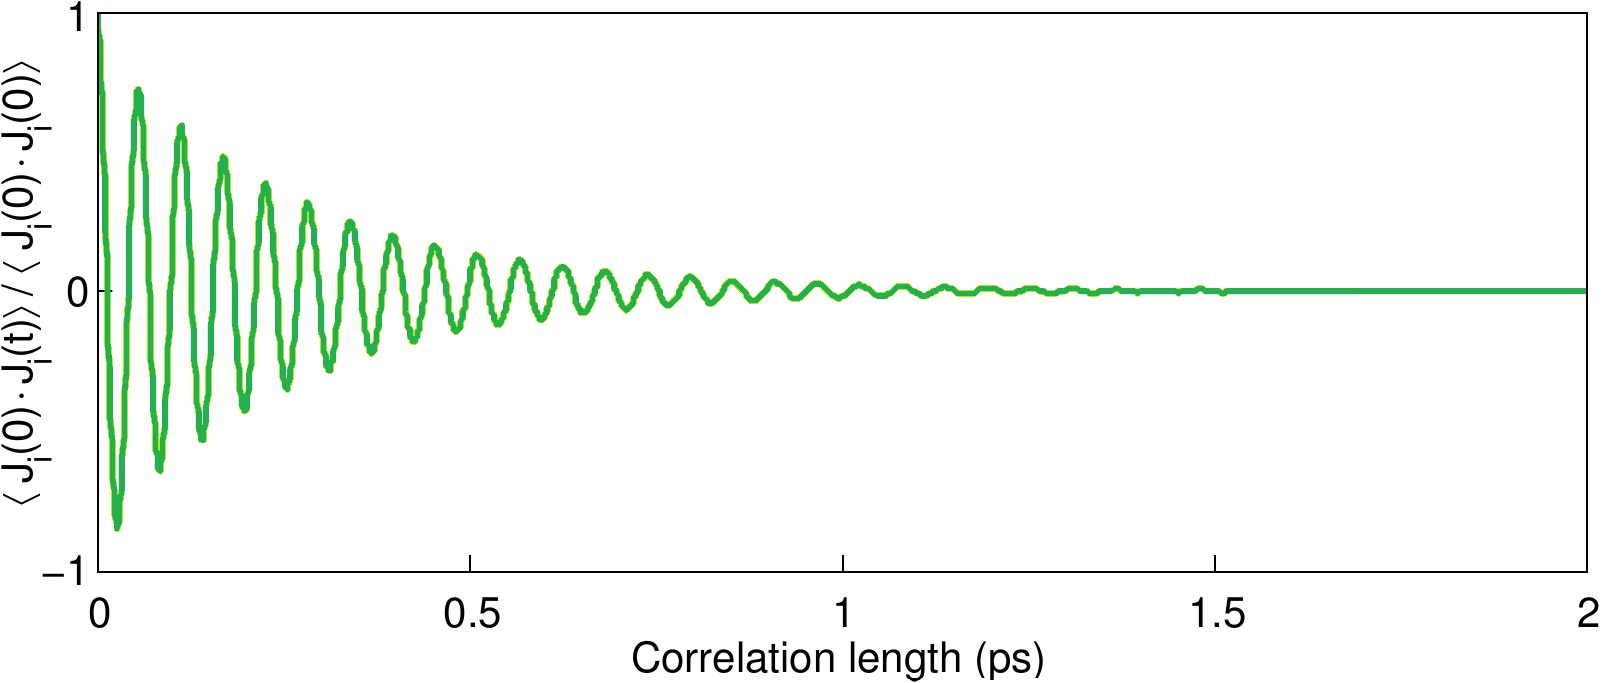
\includegraphics[width=\linewidth]{Figures/gk_acf.png}
\caption{Normalised ACF. Correlation is taken over a longer length than shown on this plot (100 ps), however the function decays to less than 1\% of its initial value at 2~ps. It continues to oscillate about zero, with a positive average value.}
\label{fig:gk_acf}
\end{figure}

The auto-correlation is obtained over the net heat flux series in each crystallographic direction, for a timescale up to a chosen correlation length.
~
\begin{equation}
ACF_i = \left \langle J_i(0) \cdot  J_i(t) \right \rangle,
\label{acf-j}
\end{equation}
~
where $i$ specifies direction, $J$ is heat flux, and $t$ is the correlation length. The integral of heat flux ACF is proportional to thermal conductivity via the Green-Kubo equation (see Figure~\ref{fig:gk_int} and Equation \ref{gk-int}), 
~
\begin{equation}
\kappa_i = \frac{V}{k_{B}T^{2}} \int_{0}^{\infty} \left \langle J_i(0) \cdot  J_i(t) \right \rangle dt ,
\label{gk-int}
\end{equation}
~
[[[I am using ``k''s and ``kappa''s to represent \tc, kappa here and k earlier?]]] where $V$ is the simulation cell volume, $k_B$ is the Boltzmann constant, and $T$ is the average temperature of the system. In this study we use Green-Kubo results as an independent check on the direct method, as they do not have the same finite size-effects. Obtaining a converged conductivity result simply depends on using a large enough cell volume / number of atoms. 

\begin{figure}[h]
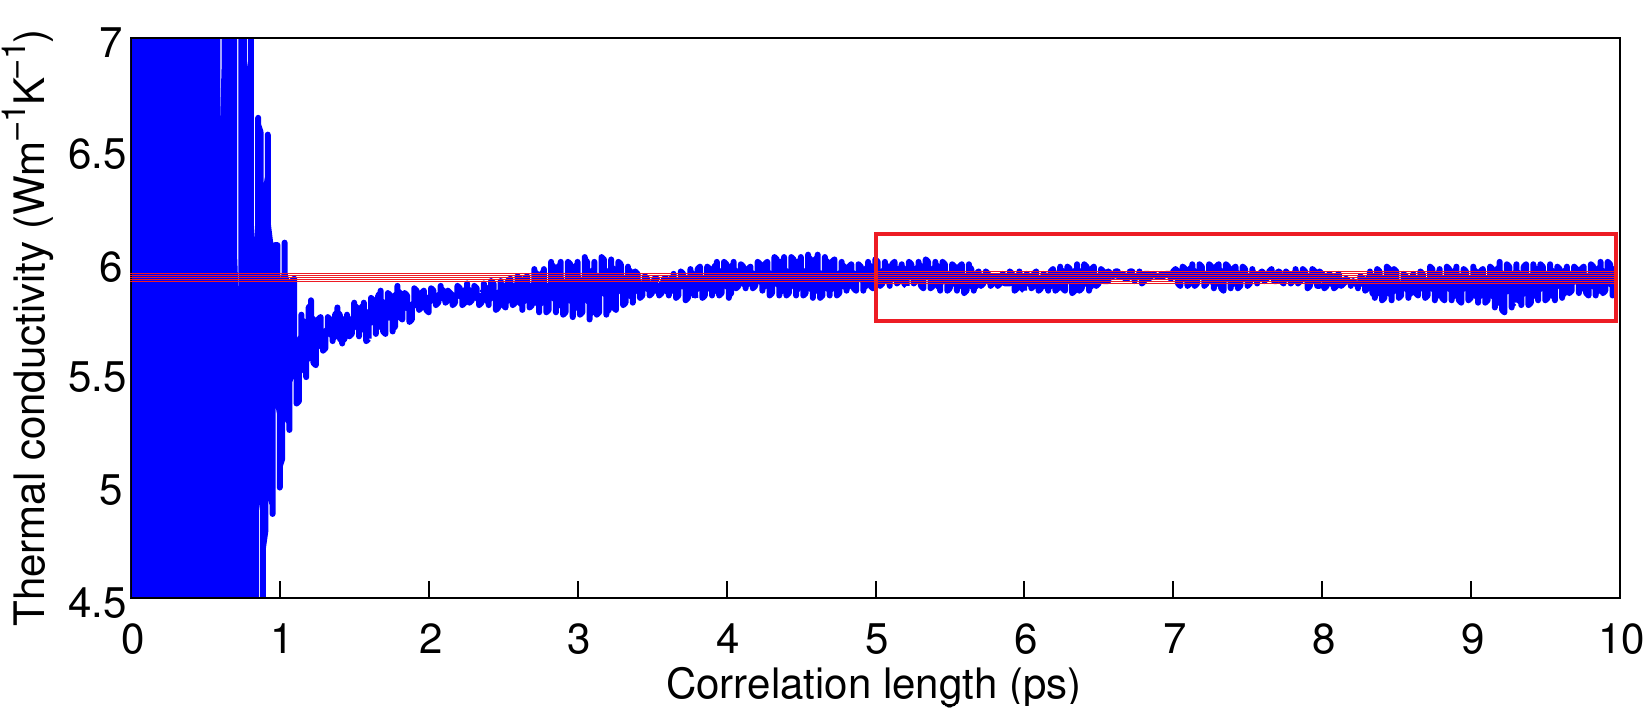
\includegraphics[width=\linewidth]{Figures/gk_int.png}
\caption{Integrated ACF, multiplied by constants to get thermal conductivity. Large variation in the first 1 ps corresponds to the correlation time where the ACF is unconverged (still decaying / large oscillations). Thermal conductivity is averaged from correlation time of 5~ps - 10~ps (region in red box).}
\label{fig:gk_int}
\end{figure}

The individual integrals obtained from the Green-Kubo show variation from the average combined integral on the order of the mean. Many simulations from different intital temperature conditions are required in order to ensure good sampling of conductivity, as well as ensuring the computation time for each is long enough for convergence. This makes Green-Kubo a computationally expensive method, especially for large systems.

The ACF should decay to zero as correlation time tends to infinity, however noise in the ACF prevents this. This will ultimately cause the integral to diverge/drift on long timescales. \citet{Howell2012} fits a series of exponential decays to their ACF, forcing the expected decay to zero and subsequent (constant) integral convergence. This is represents a significant improvement on the conductivity estimate at long correlation lengths, but is mostly similar with the un-fit integrals early in the correlation. (INTEGRAL DRIFT FIGURE, JUST THE ONE INTEGRAL FOR 100PS)

(STACKHOUSE 2010 REFERENCES Volz and Chen 2000; Sun and Murthy 2006)



%---------------------------------------
\subsection{Other}
%---------------------------------------
(3) Anharmonic lattice dynamics \citep{Tang2009}. %(BTE)CHERNATYNSKIY and PHILLPOT 2010?
\\
(4) Combined quasiharmonic lattice dynamics and molecular dynamics method \citep{DeKoker2009}.



%-----------------------------------------------------------
\section{Previous work}
%-----------------------------------------------------------

%---------------------------------------
\subsection{Method comparison}
%---------------------------------------

%---------------------------------------
\subsection{Finite-size effects}
%---------------------------------------
Should this section be interspersed into when FSE are mentioned in methods?

%-------------------
\subsubsection{STUFF THAT MIGHT BE WRONG BECAUSE FSE?}
%-------------------










%%-------------------
%\subsubsection{Parameter drift/convergence}
%%-------------------
%We ensure all calculations are run for a sufficient length of time for the conductivity value to converge. When conductivity fails to converge it means either the simulations needs to be run for longer (unlikely with our nanosecond-scale classical calculations), or the system temperature has drifted. When NVE simulations are run for a long time there is noticable drift in the average system temperature (due to numerical approximations in the equation of motion), which in turn causes drift in the computed conductivity.

%NPT-NVT-NVE PROCESS



